\subsubsection{Service Checks und deren / ihre Realisierung / Ausführung / (Überprüfungs)Methoden}

Dienste, die im Netzwerk zur Verfügung stehen (Netzwerkdienste), wie ein Web- oder FTP-Server, lassen sich einfach / simpel direkt über das Netz auf ihren Zustand (hin) überprüfen /  testen.
Hierfür muss dem entsprechende Plugin lediglich die Netzwerkadresse mitgeteilt werden, siehe Abbildung \ref{check-http} als beispielhafte Überprüfung eines Webservers.

\begin{figure}[ht]
	\centering
	   \fbox{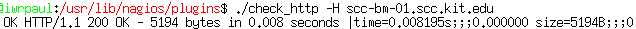
\includegraphics[width=0.85\textwidth]{bilder/check-http.png}}
		\caption{Beispielhafte manuelle Ausführung eines netzwerkbasierenden Servicechecks / HTTP Server Check}
		\label{check-http}
\end{figure}

(Bitte beachten, dass das Plugin immernoch auf dem Nagios Server ausgeführt wird / sich immernoch auf dem Nagios Server befindet)

Dienste, die sich nicht standardmäßig / ohne weiteres / ohne weitere Anpassung(en) über das Netzwerk überprüfen lassen, wie die Kapazität einer Festplatte auf einem entfernten Server(, das (Laufen) eines Prozesses) oder die Durchsuchung einer Logdatei nach bestimmten (Stop)wörtern.

Nagios bietet verschiedene Möglichkeiten an solche Dienste /  Services zu überprüfen:

\begin{figure}[ht]
	\centering
	   \fbox{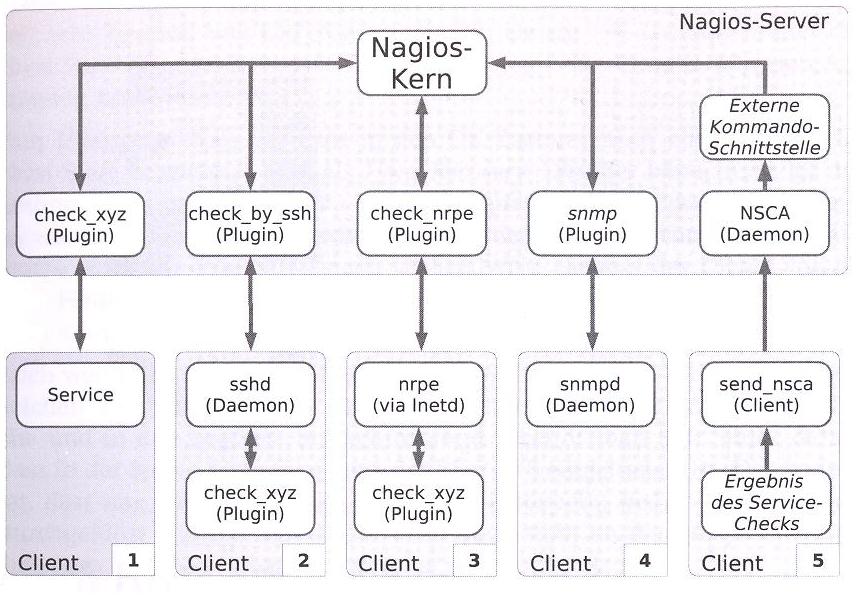
\includegraphics[width=0.85\textwidth]{bilder/nagios-kern.png}}
		\caption{Verschiedene Überwachungsmöglichkeiten von Nagios}\footnote{Quelle: \cite{Barth08} S. 98}
		\label{nagios-kern}
\end{figure} 

\textit{Hier die Zahlen als Wort oder Ziffer stehen lassen?}

\paragraph{Variante / Methode / Client 1}

Der zuvor, in Abbildung \ref{check-http}, gezeigte / abgebildete Test eines netzwerkbasierenden Dienstes wird im obigen Bild mit dem Client-Rechner (mit der Nummer) 1 realisiert.
Die Überprüfung von nicht netzwerkbasierenden Diensten soll mit den restlichen Client-Rechnern exemplarisch aufgezeigt werden.

\paragraph{Variante / Methode / Client 2}

Falls es sich beim Client um ein Unixderivat handelt, ist der entfernte Zugriff auf diesen Client per SSH\footnote{Durch eine Secure Shell (SSH) kann man sich eine verschlüsselte Netzwerkverbindung zum entfernten Rechner aufbauen.}-Dienst möglich.
Dazu muss auf dem Client ein SSH-Benutzerkonto angelegt sein, mit dem sich Nagios anmelden kann und die öffentlichen Schlüssel (zwischen Nagios Server und Client) ausgetauscht werden, damit keine passwortabhängige Benutzerauthentifizierung (Eingabe von PW) notwendig ist.
Danach können lokale Ressourcen, wie Festplattenkapazität oder Logdateien mit dem entsprechenden Plugin direkt auf dem entfernten Rechner überwacht werden.
Damit der Client diese Plugins verwenden kann, müssen sich die gewünschten Plugins (auch) auf dem Client (lokal) befinden.
Eine beispielhafte Verwendung mit dem dafür gedachten Nagios Plugin \pictext{check\_by\_ssh} (von dieser Überwachungsmethode) wird in Abbildung \ref{check-ssh} gezeigt.

\begin{figure}[ht]
	\centering
	   \fbox{
\includegraphics[width=0.85\textwidth]{bilder/check_by_ssh.png}}
		\caption{Beispielhafte manuelle Ausführung eines Servicechecks über SSH}
		\label{check-ssh}
\end{figure}

(Hier beachten, dass kein Passwort abgefragt wird, daher zuvor Schlüsselaustauschen)

\paragraph{Variante / Methode / Client 3}

Eine alternative Möglichkeit solche Dienste auf entfernten Rechnern zu überwachen, ist durch den sogenannten Nagios Remote Plugin Executor (kurz NRPE).
Hier muss auf dem Client (extra) ein "`Agent"' installiert werden, welcher einen (TCP)-Port öffnet und auf diesem auf Anweisungen durch den Nagios Server horcht.

Der Nagios Server kann diese Anforderungen über das (dafür gedachte) Plugin \pictext{check\_nrpe} an den Client verschicken.
Ein Aufruf dieses Plugins ist dem des \pictext{check\_by\_ssh} Plugins, siehe dazu Abbildung \ref{check-ssh}, sehr ähnlich.

Der Nachteil dieser Variante ist ein zusätzlich geöffneter Port und der höhere / erhöhte Aufwand beim Installieren des Agenten im Gegensatz zum (vermutlich /meistens) bereits laufendem SSH-Dienst.
Zusätzlich gibt es nur die Möglichkeit die Anfragen auf diesem Port auf bestimmte IPs zu beschränken, jedoch nicht den Zugriff durch ein Passwort zu sichern.
Dafür beschränkt sich der NRPE (lediglich) auf die auf dem entfernten Client liegenden Nagios Plugins und kann nicht System- bzw. Benutzerkommandos aufrufen, wie bspw. das \pictext{rm} Kommando zum Löschen von Dateien, welches durch den Einsatz von \pictext{check\_by\_ssh} standardmäßig möglich wäre.
Daher könnte die SSH Variante (wenn unbehandelt PATH, user einschränken) fatale Folgen nach sich ziehen, wenn es ein Angreifer schafft die Kontrolle über den Nagios Server zu erlangen.
Beide Verfahren (hingegen) unterstützen die Verschlüsselung des Datenaustausches untereinander.

\paragraph{Variante / Methode / Client 4}
Diese Variante wird nur grob angerissen / kurz / verkürzt behandelt, da sich diese Arbeit hauptsächlich mit der Überwachung von Servern beschäftigt und nicht von Netzwerkkomponenten wie Switches oder Router, die nur per SNMP überwacht werden können, wenn mehr Informationen als eine schlichte Erreichbarkeit überprüft / gesammelt werden soll.

Barth schreibt über diese Variante / Überwachungsmethode:
\begin{quote}"`Mit dem Simple Network Management Protocol SNMP lassen sich ebenfalls lokale Ressourcen übers Netz abfragen [...]. Ist auf dem Zielhost ein SNMP-Daemon installiert [...] kann Nagios ihn nutzen, um lokale Ressourcen wie Prozesse, Festplatten oder Interface-Auslastung abzufragen."' \begin{flushright}\cite{Barth08} S. 101\end{flushright}\end{quote} 

Durch SNMP kann auf die strukturierte Datenhaltung der MIB\footnote{Die Management Information Base (MIB) dient als SNMP-Informationstruktur und besteht aus einem hierarchischen, aus Zahlen aufgebauten Namensraum. Ähnliche Struktur wie andere hierarchische Verzeichnisdiensten wie DNS oder LDAP. Quelle: \cite{Barth08} S.233} in den entfernten Netzwerkknoten zugegriffen werden.

\begin{center}
TODO: SNMP MIB?
\end{center}



Man unterscheidet zwischen aktiven und passiven Checks.
\paragraph{passive}
asynchron!
Bei passiven Tests führt der zu überwachende Computer das statuserzeugende Ergebnis selbst aus und sendet es über ein Plugin zum Nagios Server.
Hierfür muss das Testprogramm bzw Script und das entsprechende Plugin \pictext{send\_ncsa}, welches zum Versenden der Informationen zuständig ist, auf dem Host vorhanden sein.
Auf der anderen Seite muss der \pictext{NSCA} (Nagios Service Check Acceptor) als Dämon gestartet sein, damit die übermittelten Ergebnisse entgegengenommen werden können.
\begin{figure}[ht]
	\centering
	   \fbox{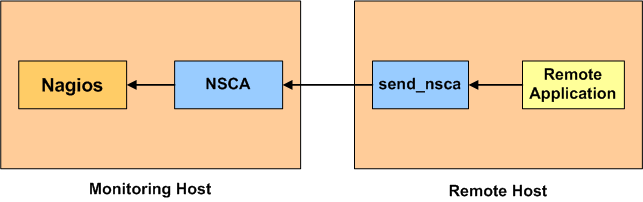
\includegraphics[width=0.85\textwidth]{bilder/nsca.png}}
		\caption{Passive Checks mit NSCA}\footnote{Quelle: http://www.nagios.org/images/addons/nsca/nsca.png}
		\label{passivchecks}
\end{figure}


\begin{figure}[ht]
	\centering
	   \fbox{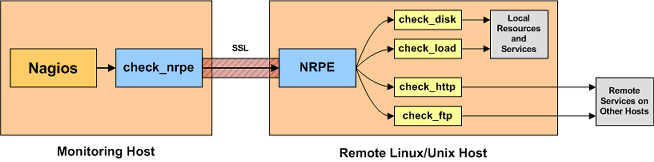
\includegraphics[width=0.9\textwidth]{bilder/nrpe.png}}
		\caption{Aktive Checks mit NRPE}\footnote{Quelle: http://www.nagios.org/images/addons/nrpe/nrpe.png}
		\label{aktivchecks}
\end{figure}
\begin{itemize}
\item Kurz agenten, zeigen auf f. Kapitel -> SNMP erklären (MIB, OID) Sicherheitsrisiko
\end{itemize}

\subsubsection{Konfigurationsdateien?}
\begin{itemize}
\item Wie/wo werden Hosts eingetragen -> hostgroups
\item Service Definitionen -> mit Host verbinden
\item Wer wird wann wegen was wie benachrichtigt -> contacts
\end{itemize}